\section{Durchführung}
\label{sec:Durchfuehrung}
\subsection{Versuchsaufbau}
Der Versuchsaufbau besteht aus einem 50l Szintillatortanke und einer Schaltung um die detektierten Myonen zu messen.
An dem Szintillatortank ist auf beiden Seiten ein Photomultiplier angebracht.
Die Photomultiplier sind zum einen an eine Hochspannungsquelle für ihren Betriebsstrom angebracht und zum anderen an eine Schaltung um die Signale auszulesen.
Jeder Photomultiplier ist jeweils mit einer Verzögerungsleitung und einem Diskrimiator verbunden.
Nach dem Diskriminator werden die beiden Leitungen aus den beiden Photomultipliern wieder in einer Koinzidenzschaltung zusammengeführt.
Von der Koinzidenzschaltung werden zeitgleich 3 Signale weitergeleitet.
Zwei dieser Signale führen jeweils in eine ''Und''-Schaltung und das dritte der Signale passiert eine Verzögerungsleitung (30 ns) die anschließend in einen Monoflop führt.
Wenn der Monoflop kein Signal bekommt legt er eine Spannung auf das eine ''Und''-Gatter und wenn ein Signal einfällt bespeist er das andere ''Und''-Gatter.
Beide ''Und''-Gatte sind jeweils mit einem Impulszähler verbunden und mit einem Input des Time-Amplitude-Converter (START und STOP Input).
Die beiden Impulszähler dienen dazu die Signale der einfallenden und auslaufenden Myonen zu zählen um festzustellen wieviele Myonen im Detektor zerfallen.
Zuletzt wird das Signal für die einfallenden Myonen in den START Input des TAC und das Signal für die auslaufenden Myonen in den STOP Input des TAC geleitet.
Der Output des TAC wird mit einem Multi-Channel-Analyser am Computer ausgelesen.
Neben dieser Schaltung ist noch ein Doppelimpulsgenerator an der Koinzidenzschaltung angebracht um die Geräte zu kalibrieren.\ref{fig:schaltbild}
\begin{figure}[H]
    \centering
    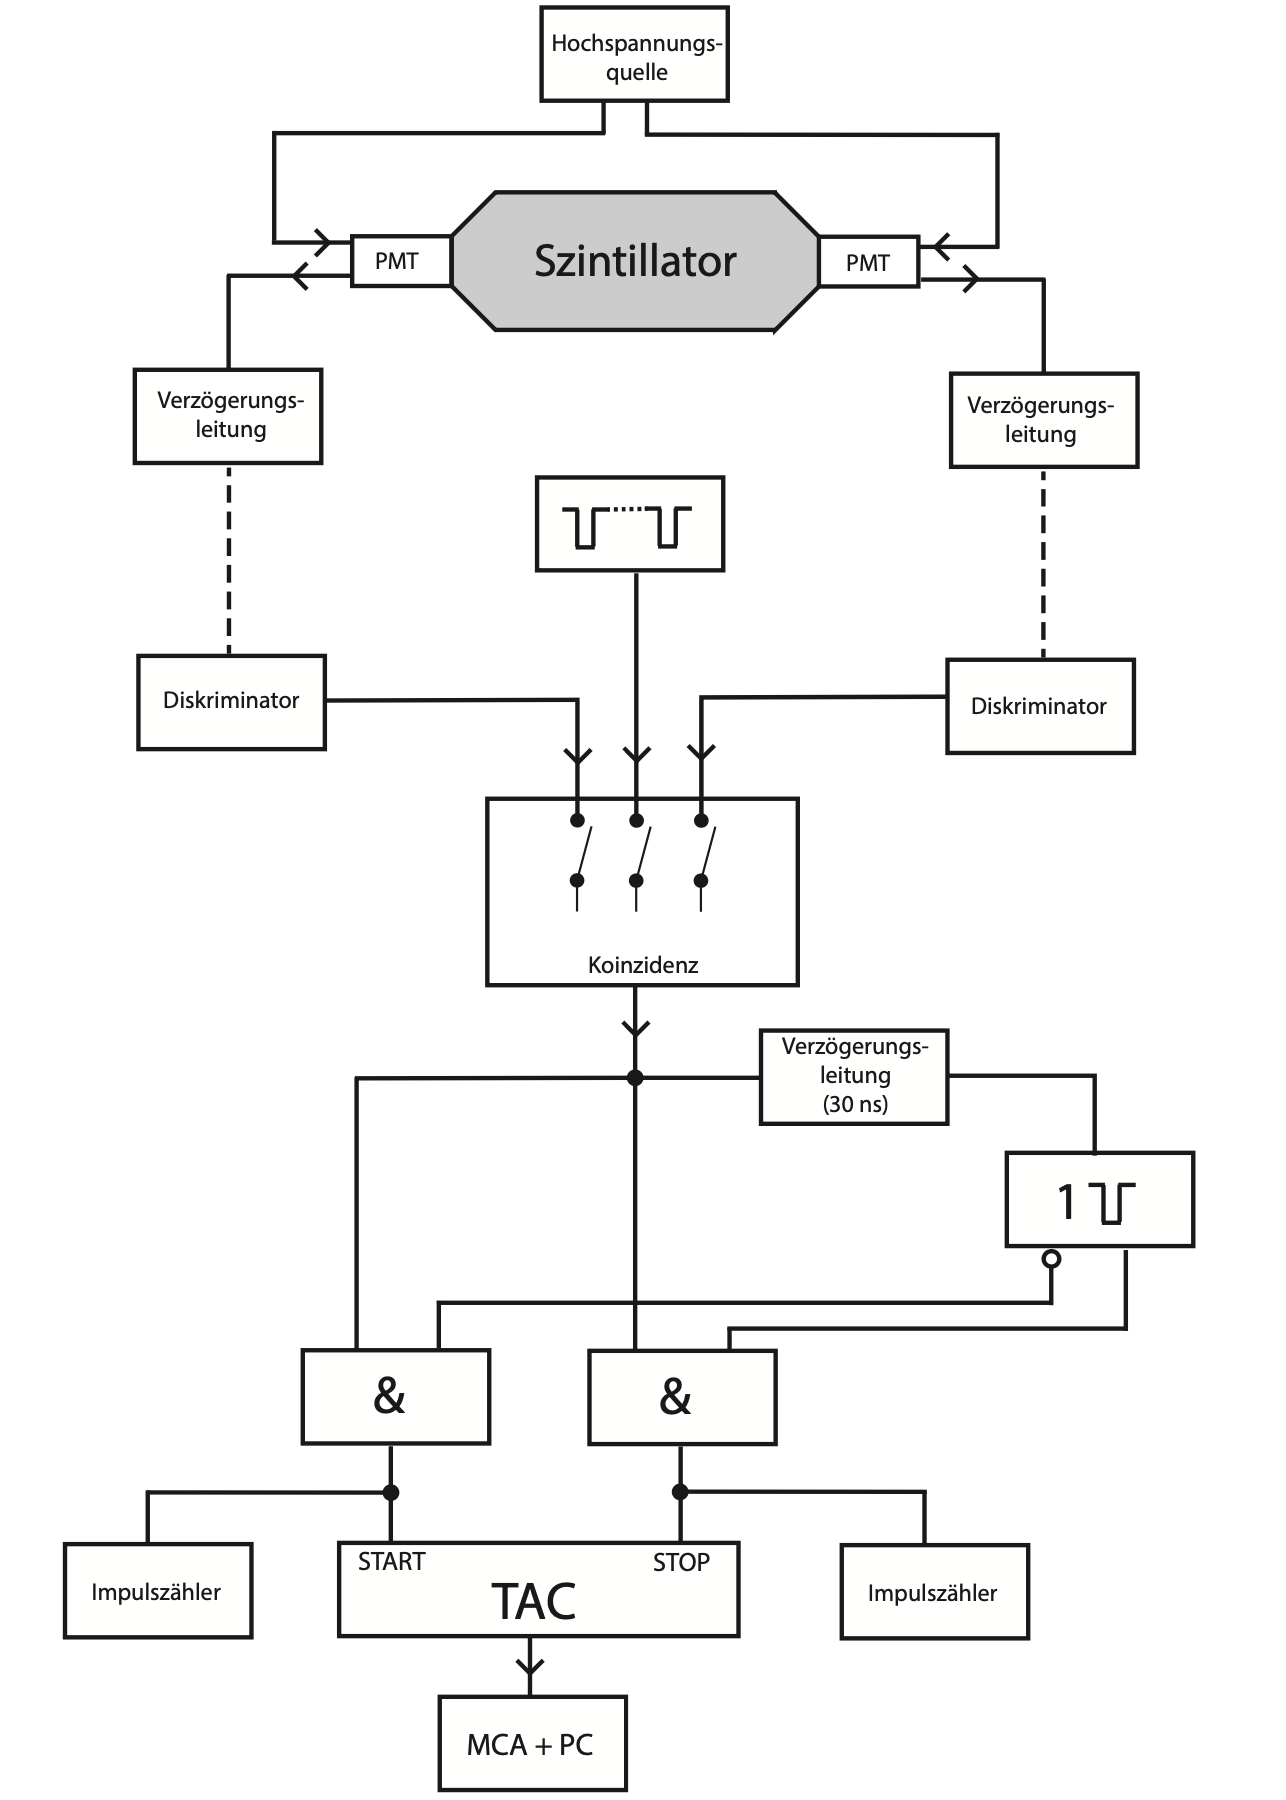
\includegraphics[width = 0.75\textwidth]{./bilder/Schaltbild.png}
    \caption{Blockschaltbild des Versuchsaufbaus \cite{anleitung}}
    \label{fig:schaltbild}
\end{figure}
\subsection{Versuchsvorbereitung}
Zunächst wurden mit dem Oszilloskop die Ausgangsimpulse der Photomultiplier vermessen um zu testen ob die PMT richtig arbeiten.\\
Um die Photomultiplier an beiden Seiten der Tanks zu kalibrieren muss bei beiden Multipliern die gleiche Anzahl an Impulsen gemessen werden.
Dazu wird die Pulsdauer auf $\Delta t = \SI{10}{\nano\second}$  eingestellt.
Daher werden sie durch das anpassen der Schwellspannung in den Diskriminatoren so eingestellt dass ca 30 Impulse pro Sekunde gemessen werden.
Über 10 Sekunden werden die Impulse gemessen und die Schwellspannung so angepasst dass 300 Impulse detektiert werden.


\subsection{Versuchsdurchführung}